    \chapter{Methodology}
       \section{SOFTWARE DEVELOPMENT APPROACH}
       Agile development is a software development approach that emphasizes incremental progress and rapid cycles. It involves releasing small increments of functionality that build upon previous versions. Thorough testing is conducted for each release to ensure software quality. Agile is often employed for time-critical applications. Although this project is not time-critical this model seems to be the most optimal and practical in our case.
       \begin{figure}[hbt!]
           \center{
               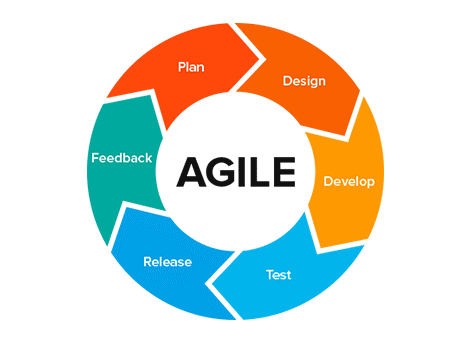
\includegraphics[width=0.75\textwidth]{./img/agile.png}
               \caption{Agile Model for Software Development}
               \subcaption*{\textit{source: \textcolor{blue}{https://mobilelive.medium.com/agile-development-a-comprehensive-guide-for-the-modern-era-d2fe9ae7b395}}}
           }
       \end{figure}
       
       \section{Implementation}

       \subsection{Data Collection}
       Datas of Nepali Text will be collected from different nepali news and governmental websites for training.
       
       \subsection{Data Preprocessing}
       \subsubsection{Normalization}
       In English, we have uppercase and lowercase letters that sound the same when we speak them. Similarly, in Nepali, there are different ways to write certain vowel sounds that sound the same when spoken. For example, the words 
    %    नेपाली and नेपालि     
        are pronounced the same way, but they are written differently. This can cause confusion and mistakes in written Nepali, making the data messy. Normalization is the process of finding these differences and making sure they are all written in the same way to clean up the data.


       
        \newpage
        \justifying
        \subsection{Gantt Chart}
            \begin{figure}[hbt!]
                \center{
                    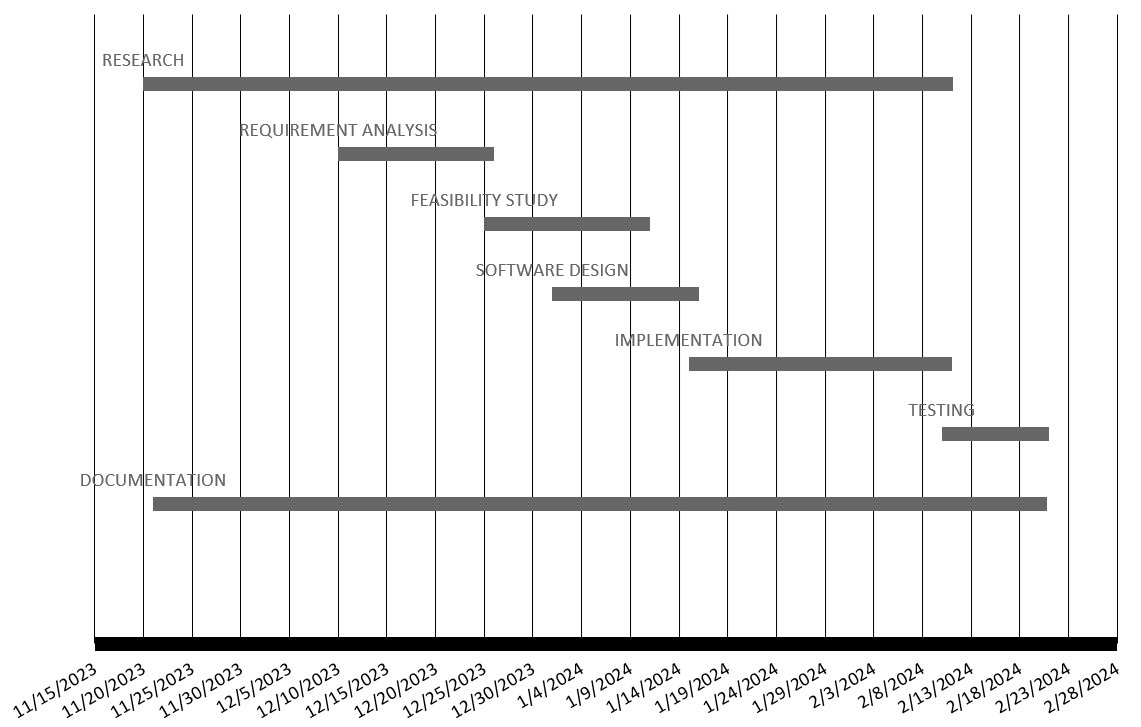
\includegraphics[width=1\textwidth]{./img/GANT_CHART.jpg}
                }
                \caption{Gantt chart}
            \end{figure}

